\subsection{Qualitatively understanding the problem}
% Explain that we want to gain insight on the influence of various parameters on the result
Due to the size of the parameter space, 
we wanted to gain a qualitative understanding of the dependence of the profile on said parameters. 
To do that, we plotted the conductivity at fixed values for all but one parameter and observed the result. 

Some of our observations were unsurprising : increasing the scattering reduces the magnitude of the conductivity for instance. 
However, at face value, the power $\nu$ has, for example, a more cryptic effect. \\

% Observe the double peak, show the fermi surface plot and interpret in terms of electron-like and hole-like regions

\begin{figure}
\centering
\begin{subfigure}{0.4\textwidth}
    \includegraphics[width=\textwidth]{example-image}
    \caption{The highly anisotropic Fermi surface exhibits both electron-like and hole-like regions (depending on the local curvature). Intuitively, we can think of them as contributing to different terms.}
    \label{fig:fermi_surface}
\end{subfigure}
\hfill
\begin{subfigure}{0.55\textwidth}
    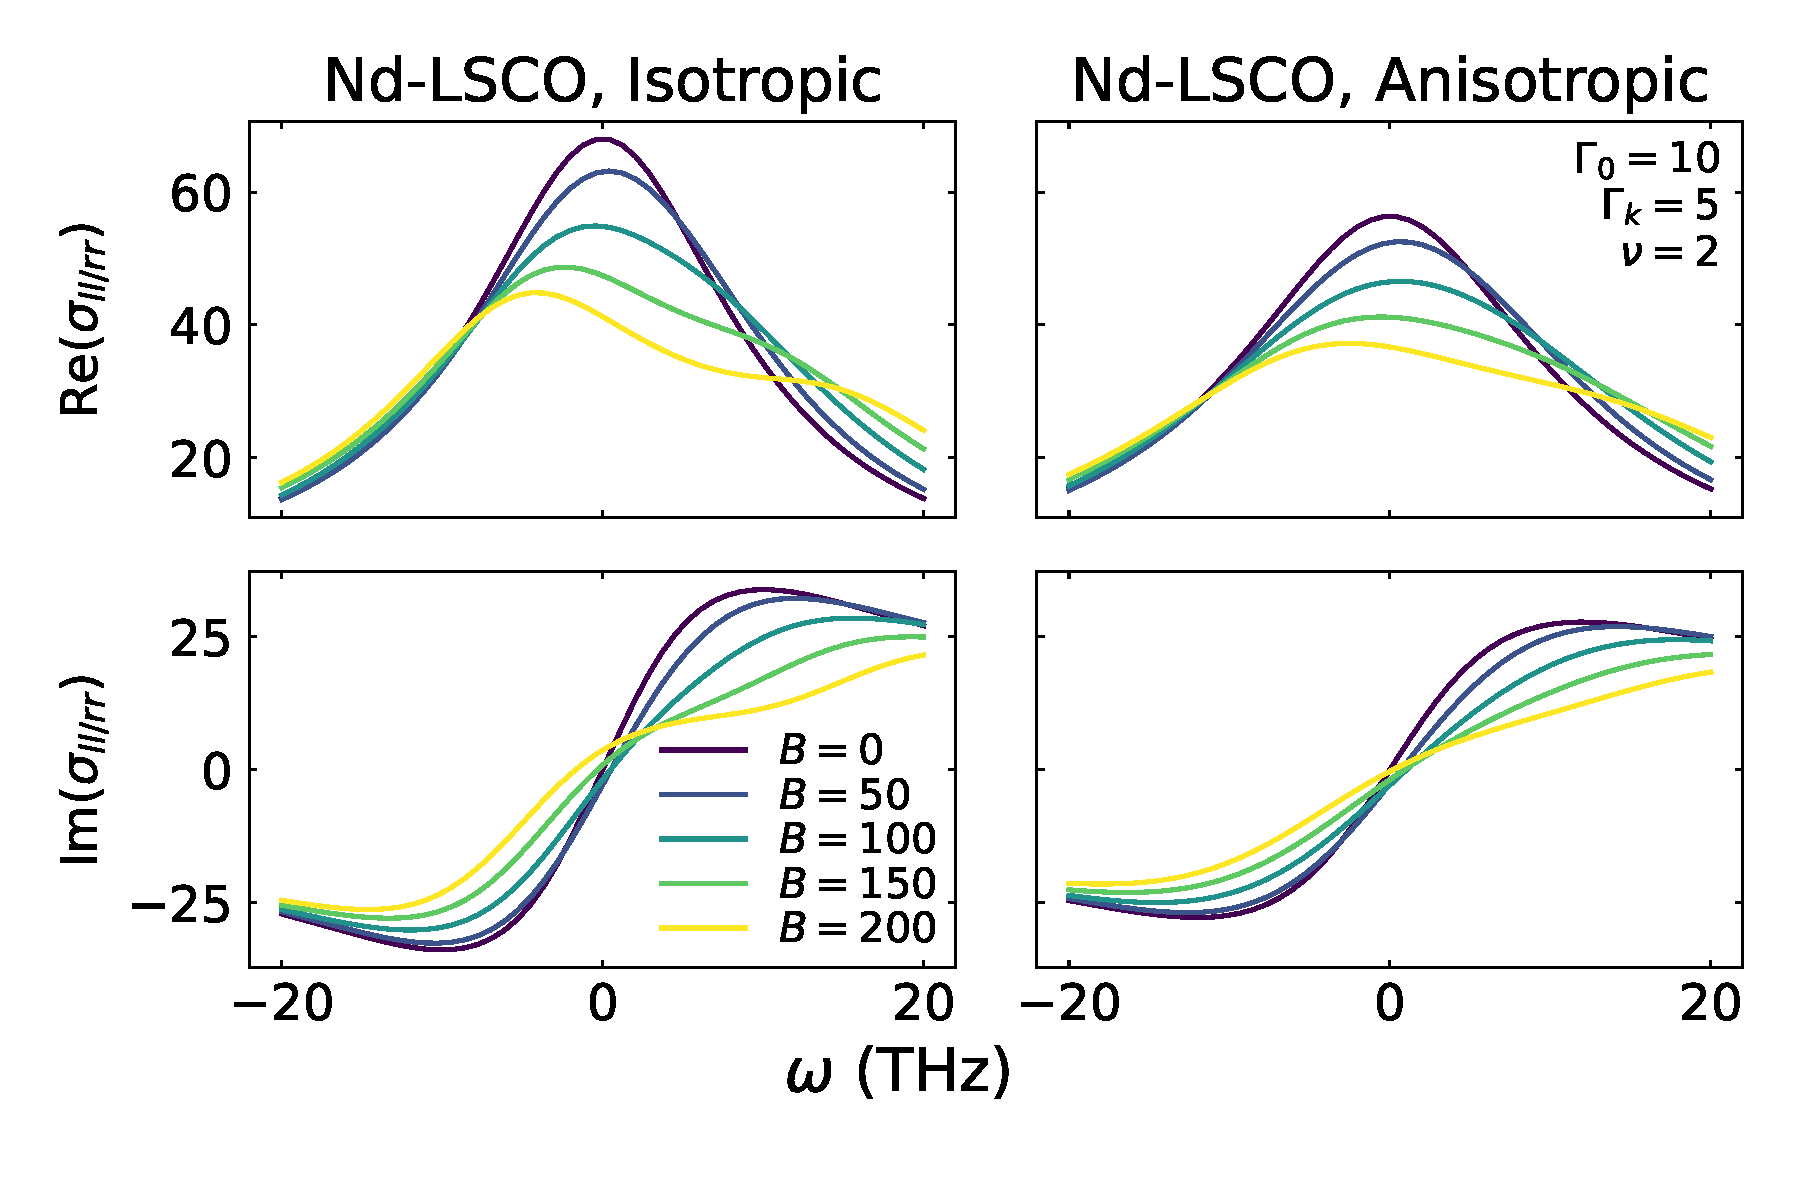
\includegraphics[width=\textwidth]{figures/NdLSCO_iso_vs_aniso_vary_field_gamma_k_5_nu_2.pdf}
    \caption{The contribution to overall conductivity of electron-like and hole-like regions of the Fermi surface can be seen as Drude peaks for charges $-e$ and $+e$ respectively.}
    \label{fig:iso_vs_aniso_vary_field}
\end{subfigure}
        
\caption{Qualitatively interpreting the dominant effects of anisotropy on the conductivity}
\label{fig:figures}
\end{figure}

Studying the influence of varying fields on the resulting conductivity profile, 
we realised that two peaks separated when it increased. 
One moving towards positive $\omega$ and the other moving towards negative values. 

This behaviour might seem puzzling at first, 
but it actually provided insight into why Chambers' formula provides us with a more accurate account than Drude 
and explained the influence of the remaining parameters on the plot. 
Indeed, if we get back to the Fermi surface (figure \ref{fig:fermi_surface}), 
we see that, due to anisotropy, its local curvature can be either positive or negative. 
Because of that, it can locally be approximated by parabolas of either sign. 
This is formally equivalent to considering that in some regions of the Fermi surface, 
the charge carriers change sign. \\

Such an observation is consistent the calculated profiles. 
Indeed, for each carrier type, we can define its cyclotron frequency. 
They will have opposite signs, meaning that as the applied field increases, 
the peaks will start drifting apart in opposite directions.

We observe that the two peaks are not equivalent, 
this can also be understood in our intuitive explanation : 
the properties of each carrier type's Drude peak are determined by the relative prevalence of one over the other on the Fermi surface. 
Therefore, their relative intensities and widths (\textcolor{red}{are we sure}) are determined by the shape of the anisotropy

% Identify the challenge in terms of 
As we can deduce from our tests in parameter space and from our interpretation of the effect, 
there are several parameters that have similar effects 
(such as an increasing $\nu$ and a decreasing $\Gamma_k$). 
This explains the trouble we had in fitting the data correctly : 
the work was still not over at that point.
